In this chapter we include an overview of the main research areas related to this thesis. The Stream Reasoning research context, to which this thesis belongs, is introduced in Section~\ref{sec:sfp}. It has the aim of unifying the Semantic Web research area, we briefly present in Section~\ref{sec:sw} and the Information Flow Processing (IFP) research one, described in Section~\ref{sec:ifp}. 

This thesis proposes \namens, an open source framework for the Systematic Comparative Research Approach. Section~\ref{sec:empirical-research} contains the state of the are of the Empirical Research in the Computer Science. It is worth to note that Software Testing and Benchmarking are the two most relevant approach to empirically evaluate software systems. For this reason we include in this Chapter an introduction about Software Testing in Section~\ref{sec:software-testing} and one about Benchmarking in Section~\ref{sec:benchmarking}.

\section{Semantic Web}\label{sec:sw}

The Semantic Web (SW) is the World Wide Web extension  that  provides a common framework to share and reuse data across applications, enterprise, and community boundaries. Tim Berners-Lee, the inventor of the World Wide Web and director of the World Wide Web Consortium (W3C), supervises the development of proposed Semantic Web standards. Nowadays, a large number of researchers and industrial partners collaborate with the W3C to the Semantic Web research.\\
\begin{center}
"The Web can reach its full potential if it becomes a place where data can be processed by automated tools as well as people". [W3C, 2001].
\end{center}

\noindent The Tim's definition above highlights the Semantic Web vision of the new era, the Web 3.0,  where the information can be processed and manipulated by machines. SW can give to the information a well defined meaning. The way to reach this goal is adding a new layer of meta-data to the existing documents and data. The semantic definition of data and documents enables to understand and respond to complex human needs. The outcome of this vision is an evolution to a new Web, where intelligent agents can browse data on behalf of the user and make knowledge easier to be reached.


\begin{figure}[tbh]
  \centering
	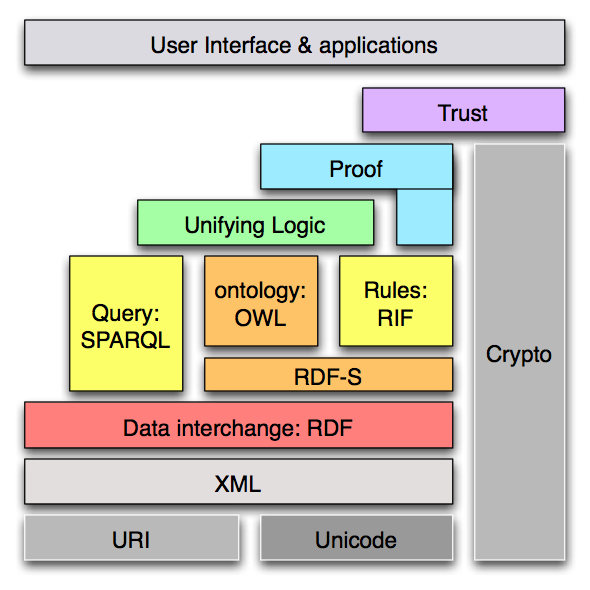
\includegraphics[width=0.75\linewidth]{images/semantic_web_stack}
	\caption{Semantic Web Stack} 
  	\label{fig:semantic-web-stack}
\end{figure}
 

Semantic Web world involves several technologies. Due to the complexity of the concept, the W3C proposed a layered approach, presented in Figure~\ref{fig:semantic-web-stack}, in which each level contains a set of standards for semantic technologies.
\pagebreak

The first level of the Semantic Web stack includes two standards of World Wide Web:
\begin{itemize}
\item  The Uniform Resource Identifier (URI)  and Internationalised Resource Identifier(IRI), which guarantee the interoperability between heterogeneous systems. They stay at the lowest level.
\item  The Unicode standard is a character encoding standard to represent and manipulate text in many languages.
%\item  The eXtensible Markup Language (XML) is a wide-spread standard for data exchange in the Web that states the basic syntax level. In the SW stack it is build on top of URI and Unicode. 
\end{itemize}

On the top of them, the basic syntax level is provided by the eXtensible Markup Language (XML), a wide-spread standard for data exchange in the Web. The XML parsers support the lower-level syntax checking of the Semantic Web documents. However, the XML standard is not enough for the data exchange in the semantic web, because it is suited to recognize syntax, but not equivalent models. For this reason, three middle layers are required to ensure the semantic interoperability:
\begin{itemize}
\item The Resource Description Framework (RDF) is a language for expressing data models, which are usually encoded in XML.
\item RDF Schema (RDFS) defines a vocabulary for describing classes and properties of RDF resources.
\item The Web Ontology Language (OWL) extends the RDF Schema by adding advanced concepts in order to facilitate a more realistic representation of knowledge based on the RDF resources.
\end{itemize} 

Last but not least, another important standard, which covers multiple layers, is the official Semantic Web Query Language: SPARQL,  the official query language for the SW and a W3C Recommendation since January 2008. 

In the following subsections, we will present some basic concepts of the Semantic Web:  RDF in Subsection~\ref{sec:rdf},  OWL in Subsection~\ref{sec:owl}, Linked Data in Subsection~\ref{sec:ldata} and SPARQL language~\ref{sec:sparql}

Finally, technologies at the top layers are not yet standardized or implemented:
\begin{itemize}
\item The Rule Interchange Format (RIF) or SWRL allows knowledge inference from existing data.
\item Cryptography is important to verify if semantic web statements are coming from trusted source.
\item Trust involves the trustworthiness and reliability of the data.
\item User interface is the final layer that will enable humans to use Semantic
\end{itemize} 

\subsection{Resource Description Framework (RDF)}\label{sec:rdf}

The Resource Description Framework (RDF) is the W3C standard for data interchange on the Semantic Web~\cite{rdfconcepts}. Through RDF we can describe a conceptual model of information in any given domain of knowledge. Information is represented in the statement form subject-predicate-object. In general a statement is composed by three different resources, indeed statements are also called triples and set of triples is called a graph. More formally, we provide the definition of RDF triples and RDF graphs:

\textbf{Definition}: Let $I$, $B$ and $L$ be three pairwise disjoint sets, defined as IRIs, Blank Nodes and Literals, respectively. A triple \[ (s, p, o) \in (I \cup B) × I × (I \cup B \cup L) \] is  an \textit{RDF triple}, while a set of \textit{RDF triples} is called an R\textit{DF grap}h.

Notice that:
\begin{itemize}
\item IRIs are Internationalized Resource Identifiers, an extension of Uniform Resource Identifiers (URIs) that enlarge the character set from ASCII to Unicode.  IRIs provide the linking structure of the Web and allow a globally connection between any different \textit{RDF graph}.
\item Literals are constant values, represented by character strings, which can be associated to a XML Schema datatype. 
\item Blank nodes represent anonymous resources, usually resources that group a number of other resources and which are never directly referenced.
\end{itemize}

The Resource Description Framework has several possible representations.

The most natural representation for triples is the N3 notation, which consists in explicit each triple in the form:
 \[<subjectIRI> <predicateIRI> <objectIRI>/objectLiteral\]
 
The official syntax for RDF models is RDF/XML, which is an XML dialect for describing RDF. Many applications exploit the XML Language in the Web, indeed the XML document validation of the basic syntax of RDF/XML is possible through the RDF/XML standard schema. 

\begin{lstlisting}[language=XML, caption=An example of a simple RDF/XML document:, label=code:rdf]
<rdf:RDF xmlns:rdf="http://www.w3.org/1999/02/22-rdf-syntax-ns#"
 		 xmlsn:rdfs="http://www.w3.org/2000/01/rdf-schema#"
 		 xmlns:foaf="http://XMLns.com/foaf/0.1/">
  <rdf:Description rdf:ID="marvin">
    <foaf:name>Marvin</foaf:name>
     <rdf:type>
        <rdfs:Class rdf:about="#ManicDepressiveRobot"/>
     </rdf:type>
  </rdf:Description>
</rdf:RDF>
\end{lstlisting}

The Code Snippet~\ref{code:rdf} contains an example of a simple RDF/XML document. Each RDF/XML document starts with an unique rdf:RDF element and the definition of the useful namespaces (lines 1-3). The rdf:Description tag (lines 4-9) represents an RDF Statement and it includes the subject of the statement, in our case Marvin. Inside the rdf:Description element we define two predicates: foaf:name (line 5) which contains an object literal, a string with the name of the resource; rdf:type (lines 6-8), a special predicate, which relates the individual resource to its class. In this case Marvin is an individual of the class ManicDepressiveRobot (line 7).

\begin{figure}[tbh]
  \centering
	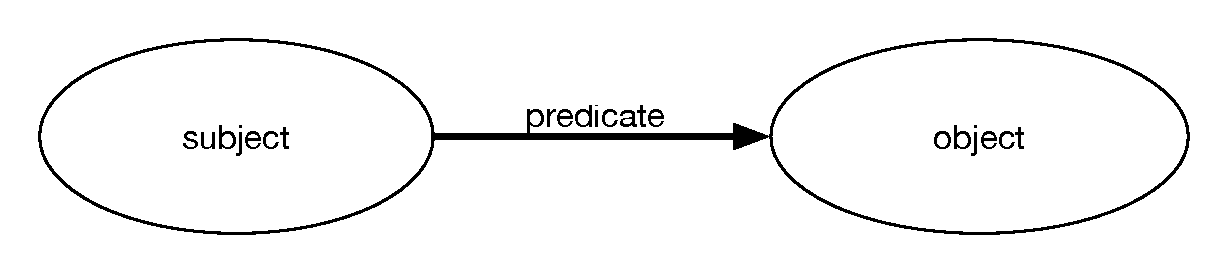
\includegraphics[width=0.75\linewidth]{images/rdf-graph}
	\caption{RDF Model Graph} 
  	\label{fig:rdf-graph}
\end{figure}

Last but not least, Figure~\ref{fig:rdf-graph} shows the graphical representation of an RDF model as RDF graph:  subjects and objects are the graph nodes and proprieties are represented as edges connecting a subject to an object. 

\subsection{RDF Schema}\label{sec:rdfs}

RDF Schema (RDFS) is a semantic extension of the RDF. It allows to describe taxonomies of classes and properties, to define groups or restrictions of resources which are related and  it enables to detail the relations between these resources. It is written in RDF and it also extends some RDF elements. Its constructs can be used to determine characteristics of other resources, such as the domains and ranges of properties.

RDFS class and property system is similar to the one of traditional Object-Oriented programming languages. RDF Schema describes properties in terms of the classes of resource to which they apply, through the domain and range properties. This property-centric approach aims of being easy-to-extend.

RDFS contains fifteen classes and the most relevant ones are:

\begin{itemize}
\item rdfs:Resource - everything in RDFS is an instance of this class.
\item rdfs:Literal  -  sub class of rdfs:Resource represents a text string
\item rdf:Property  -  sub class of rdfs:Resource and represents the properties
\item rdfs:Class    -  sub class of rdfs:Resource, it represents the type concept typical of the OO programming languages and thus it is related to the rdf:type property. Every class is an instance of rdfs:Class
\end{itemize}

It also contains sixteen properties, all instances of rdf:Property, and the most important ones are:
\begin{itemize}
\item rdf:type - used to state that a resource is an instance of a certain rdf:Class.
\item rdfs:subClassOf - used to state that all the instances of one class are instances of another.
\item rdfs:subPropertyOf - used to state that all resources related by one property are also related by another.
\item rdfs:range - used to state that the values of a given property are an instance of one or more classes
\item rdfs:domain -  used to state that any resource that has a given property is an instance of one or more classes
\end{itemize}


\subsection{$\rho$DF}\label{sec:rhodf}

Efficient data processing in SW depends on the trade off between the expressiveness of the language that describes the data and the dimension of the dataset. Nowadays, developers have to face with scalability problems, due to the enormous size of data to process. For this reason, several RDF and RDFS fragments, with good trade off between performances and expressiveness, have been proposed.

$\rho$DF~\cite{DBLP:conf/esws/MunozPG07}, is a fragment of RDFS that conserves the original semantic and covers only those vocabulary and axiomatic information that  serves to reason about the data it describes and not about the structure of the language itself. $\rho$DF comprehends:
\begin{itemize}
\item rdfs:subPropertyOf
\item rdfs:subClassOf
\item rdfs:domain 
\item rdfs:range
\item rdf:type 
\end{itemize}

Notice that w.r.t RDFS (see Section~\ref{sec:rdfs}) it does not include the rdfs:Class, which is relevant for Semantic Web ontological level, but it does not play any relevant role in the frame of RDFS deductions. A similar argument can be done for rdfs:subClassOf and rdfs:subPropertyOf reflexivity, which do not play any relevant role in the semantics and thus can be avoided without having side-effects.

\cite{DBLP:conf/esws/MunozPG07} provides the evidences that $\rho$DF reserves the normative semantics and core functionalities of RDFS. Moreover,  $\rho$DF can be considered relevant from  the Stream Reasoning research point of view, because several works in the field  has already successfully chosen it as entailment regime~\cite{DBLP:conf/semweb/UrbaniMJHB13, Liu:2014:ERS:2567948.2577323}.

\subsection{Web Ontology Language}\label{sec:owl}

The Web Ontology Language (OWL) is the W3C standard for describing rich and complex knowledge about resources, groups of resources, and relations between resources, or more formally an \textit{Ontology}. Tom Gruber define an ontology as \textit{a specification of a conceptualization}~\cite{Gruber:1993:TAP:173743.173747}. Practically, it can be a set of Description Logic axioms which tries to represent a fragment of reality. 

OWL is obtained extending the RDF Schema Language with additional language constructs and some constrain on the usage of RDF(S)  ones. The aim of these constrains is to restrain the language to a subset of First Order Logic. Different constrains define different levels of expressiveness and complexity. The W3C has standardized three different OWL dialects called Profiles\footnote{http://www.w3.org/TR/owl2-profiles/\#OWL\_2\_EL}, in Dec. 2012. In the following we present them in order of increasing level of complexity:

\begin{itemize}
\item OWL 2 EL - this profile is suitable for ontologies with a huge number of classes to manage the terminology or which include complex structural descriptions. It works well for  applications domains that have structurally complex objects. OWL 2 EL does not support negation, disjunction, and universal quantification on properties.

\item OWL 2 QL  - this profile is suitable for applications that aim to both represent database schemas  and translate reasoning into queries. It can be used as an high level database schema language, because it is realized using standard relational database technology (e.g., SQL). It also provides many of the main features necessary to express conceptual models such as UML class diagrams and ER diagrams. OWL 2 QL does not allow existential quantification of roles to a class expression, property chain axioms and equality.
\item The OWL 2 RL - this profile is tailored for applications that demand a good trade off between scalable reasoning and expressive power. Rule-based implementations of OWL 2 RL, under RDF-Based Semantics, can be used with arbitrary RDF graphs. An ideal way to enrich existing RDF data, especially when the data must be massaged by additional rules. OWL 2 RL disallows statements where the existence of an individual enforces the existence of another individual: for instance, the statement "every person has a parent" is not expressible in OWL RL.

\end{itemize}

\begin{lstlisting}[language=XML, caption=An example of a simple OWL DL RDF/XML document:, label=code:owl]
<rdf:RDF xmlns:rdf="http://www.w3.org/1999/02/22-rdf-syntax-ns#"
 xmlsn:rdfs="http://www.w3.org/2000/01/rdf-schema#"
 xmlns:foaf="http://XMLns.com/foaf/0.1/">
  <owl:Class rdf:ID="ManicDepressiveRobot">
    <rdfs:subClassOf rdf:resource="#Robot"/>
    <rdfs:subClassOf>
      <owl:Restriction>
        <owl:onProperty rdf:resource="#hasMood"/>
        <owl:minCardinality>2</owl:minCardinality>
      </owl:Restriction>
    </rdfs:subClassOf>
  </owl:Class>
\end{lstlisting}

OWL can be serialized in the RDF/XML syntax. In the Code Snippet~\ref{code:owl}, we use OWL to describe the Class of ManicDepressiveRobot, which is a SubClass of Robot that has at least two Moods. The owl:Class tag (lines 4-12) is a shortcut to represent an RDF Statement about a resource with a rdf:type of owl:Class. The subject of the statement is the resource ManicDepressiveRobot, which represents the class of individual Manic Depressive Robots. This statement has two predicates, both of the type rdfs:subClassOf. The first predicate (line 5) relates the OWL class ManicDepressiveRobot to its super-class, the resource Robot. The second predicate (lines 6-11) states that ManicDepressiveRobot is a subclass of the OWL restriction class, which contains all the individuals that are in relationship hasMood (line 8) with at least 2 resources (line 9).


\subsection{Linked Data}\label{sec:ldata}

The Linked Data concept indicates a set of best practices in publishing and connecting Semantic Web data. Bizer, the Linked Data creator, defines the term as follow:

\begin{quote}
Linked Data refers to data published on the Web in such a way that it is machine-readable, its meaning is explicitly defined, it is linked to other external readable, defined, data sets, and can in turn be linked to from external data sets~\cite{heath2011linked}.
\end{quote} 

\begin{figure}[tbh]
  \centering
	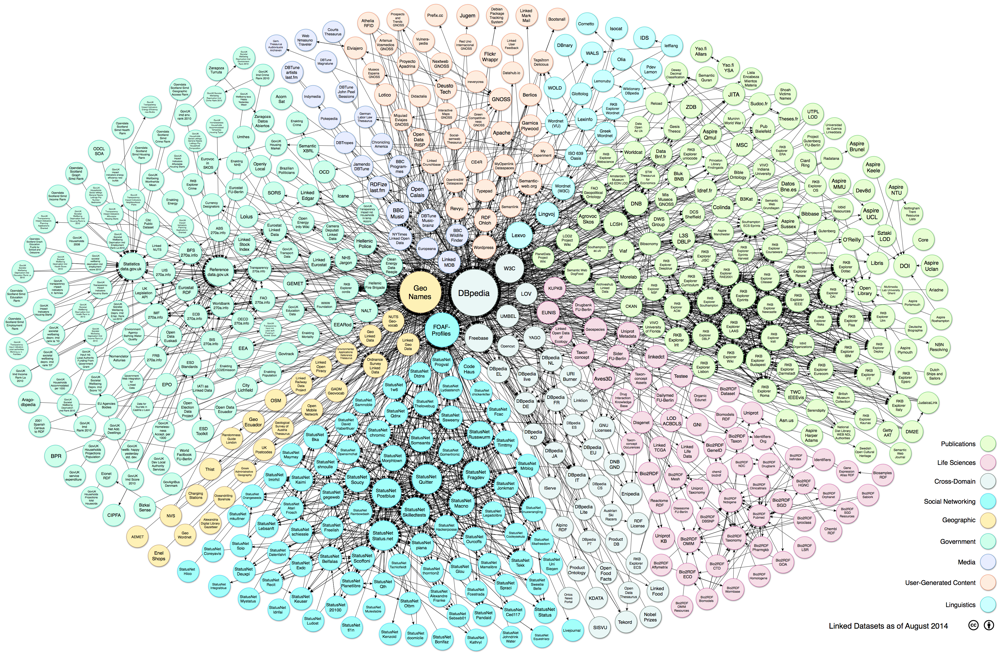
\includegraphics[width=\linewidth]{images/lod}
	\caption[Linked Data Cloud]{Linked Data Cloud of August 2014\footnote{lod-cloud.net}} 
  	\label{fig:lod}
\end{figure}

Datasets that are published according to the Linked Data principles can be navigated using Semantic Web browsers. Figure~\ref{fig:lod} presents  Linked Data Cloud updated to August 2014. It is the connected graph which comprises all the dataset published according to the LD principles. Each node of the graph represents a dataset, while each edge represents the connections between datasets.

The number datasets that follow the Linked Data paradigm is increasing every day and among the most important of them we can cite DBpedia, which wraps Wikipedia articles into a Semantic Web compliant form. Moreover, several governments, like the UK government\footnote{http://data.gov.uk/}, decide to publish their public data and connect them to the Linked Data cloud. 

\subsection{SPARQL}\label{sec:sparql}

The SPARQL Protocol and RDF Query Language (SPARQL) are, since January 2008, the W3C standard query language for retrieving data in RDF format~\cite{prudhommeaux_sparql_2008}.

The SPARQL query language was initially designed to meet the requirements identified in the RDF Data Access Use Cases and Requirements. Only successively it has been formalized through the definition of an official algebra, developed as an evolution of previous RDF query languages such as rdfDB, RDQL, and SeRQL.

Recently, W3C released a working draft describing the new version of SPARQL\footnote{http://www.w3.org/TR/sparql11-query/.}. SPARQL 1.1, this is the name of the new relase, is completely compatible with the SPARQL specification, but it has some new additional features, like aggregates, subqueries, negation and project expressions, i.e. the possibility to use expressions in the SELECT clause. These features were already part of several implementations of SPARQL, for example in the ARQ query engine. 

SPARQL is defined as a graph-matching query language to face the RDF labelled graph. The language specifies four different query variations, each of which takes a WHERE Block to describe and restrict the searched graph:
\begin{itemize}
\item SELECT query: used to extract a set of variables and their matching values, called set of mappings in the table format.
\item CONSTRUCT query: used to provide an RDF graph created directly from the results of the query.
\item ASK query: used to provide a simple boolean value expressing if there are any matches in the graph.
\item DESCRIBE query: used to extract an RDF graph based on the infor- mation related to the retrieved resources.
\end{itemize}

\begin{lstlisting}[language=SQL, caption=An example of a simple SPARQL query , keywords={PREFIX,SELECT,WHERE,ORDER,BY, LIMIT }, label=code:sparql]
PREFIX foaf: <http://xmlns.com/foaf/0.1/> 
SELECT ?person ?name
WHERE {
?person a foaf:Person.
?person foaf:name ?name }
ORDER BY ?name 
LIMIT 3
\end{lstlisting}

The code snippet~\ref{code:sparql} contains a simple example of SPARQL Select query. In general the structure of such queries (SELECT) consists of five clauses:
\begin{itemize}
\item PREFIX: The PREFIX keyword associates a prefix label with an IRI. A qualified name is a prefix label and a local part, separated by a colon, which is mapped to an IRI.
\item SELECT: The SELECT keyword specifies the form of returning variables and their combinations by introducing new variable.
\item FROM: The FROM keyword allows a query to specify an RDF dataset by reference.
\item WHERE: The WHERE keyword provides the graph pattern to match against the data graph. The graph pattern can be in different form of simple graph pattern, group graph pattern, optional graph pattern, alternative graph pattern. Different keywords can be used in this clause such as OPTIONAL (for optional patterns), UNION (for unions of patterns), FILTER (for filtering patterns).
\item Solution modifiers: this clause use different keywords like ORDER BY, LIMIT,. . . in order to modify the result of the query.
\end{itemize}

Further restrictions can be applied using keywords like FILTER, ORDER BY, LIMIT, AND, or UNION.

%\subsection{Reasoning}\label{sec:reasoning}
\pagebreak

\section{Information Flow Processing}\label{sec:ifp}

The application domain of Information Flow Processing (IFP) includes systems able to collect information flows produced by multiple, distributed sources. Such systems, called IFP Engines, process the information in a timely way, extracting new knowledge from the information flow as soon as it is collected.

\begin{figure}[tbh]
  \centering
	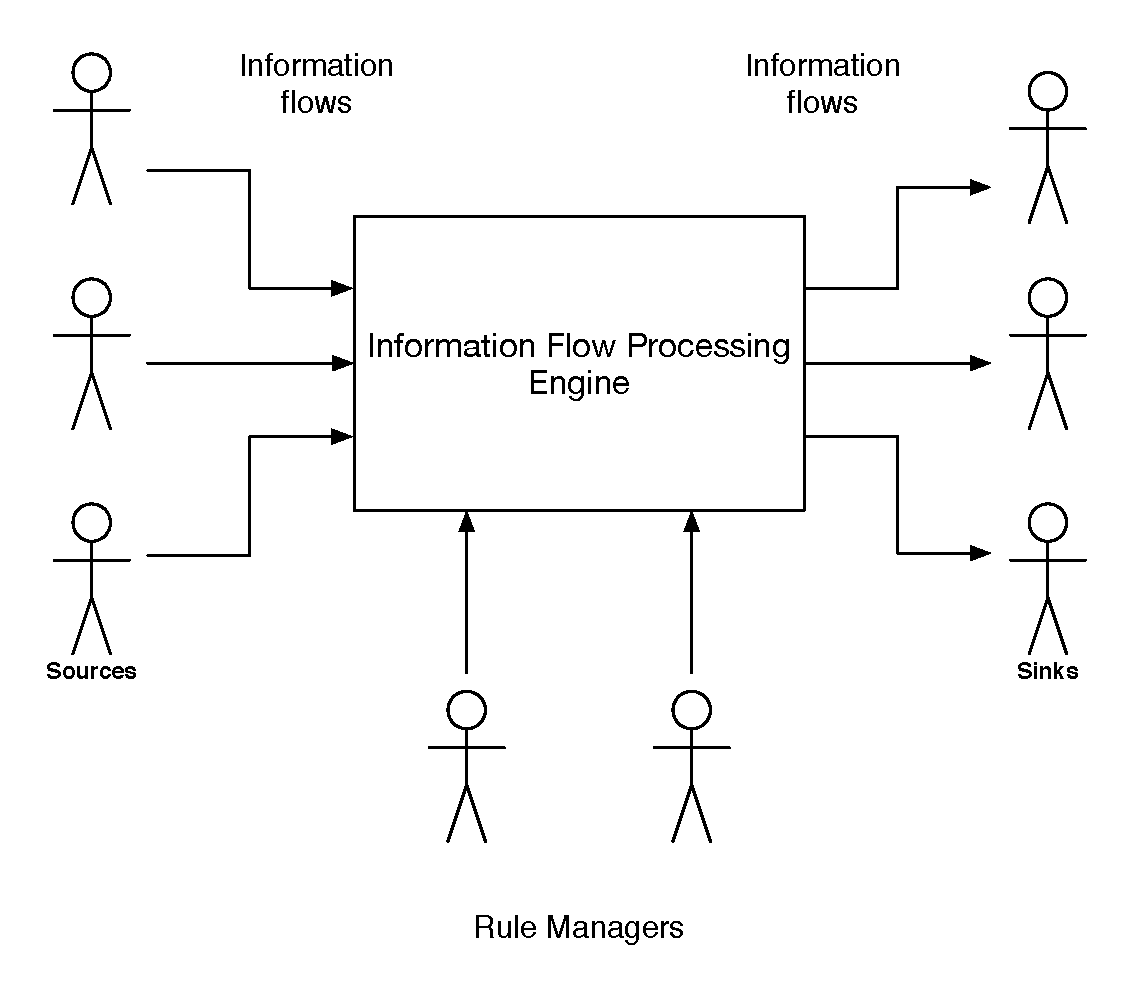
\includegraphics[width=0.75\linewidth]{images/ifp}
	\caption[IFP general Model]{The Information Flow Processing general Model proposed in~\cite{Cugola:2012:PFI:2187671.2187677} highlights the distributed and heterogeneous nature of information flows. The IFP Engine is a rule-based system that processes information flows. Practically it applies rules filtering, combining and aggregating different data flows, which have  heterogeneous domain origins, in order to produce a new information flow that will be consumed by other systems.}
  	\label{fig:ifp}
\end{figure}

An IFP Engine is \textit{capable of timely processing large amount of information, which flows from the peripheral to the center of the system} as can be seen if Figure~\ref{fig:ifp}, which shows the general IFP Engine model proposed in~\cite{Cugola:2012:PFI:2187671.2187677}. The IFP Engine receives many input information flows and it processes the flow items, as soon as they are available, through a set of processing rules. The ruleset specifies how to filter, combine, and aggregate the different flows of information. Item by item the IFP generates a new flow, which represents the output of the engine.

The research works in the IFP context have developed two main models: the Data Stream Processing Model (DSMS)~\cite{Babcock:2002:MID:543613.543615} and the Complex Event Processing (CEP) Model~\cite{Luckham:2001:PEI:515781}. 
DSMS processing is led by two concepts, the Relational Data Stream and the Window. On the other hand, CEP processing exploits the notion of event and by considering the input flow as sequence of notifications, which can be aggregated to obtain catch the semantic value of the stream.

We detail these two models of IFP respectively for DSMS in Subsection~\ref{sec:dsms} and for CEP in Subsection~\ref{sec:cep}

\subsection{Data Stream Management System}\label{sec:dsms}
The DSMS research field views the IFP problem as an evolution of traditional data processing, describing it as \textit{processing streams of data coming from different sources to produce new data streams as an output}. A Data Stream Management Systems (DSMS) extends the traditional DBMSs, in particular for the following considerations:

\begin{itemize}
\item streams are usually unbounded, while tables are not
\item assumption on data arrival order and rate can not be formulated
\item size and time constraints make hard, probable impossible, storing and processing data stream; one-time processing is the typical mechanism used to deal with streams
\end{itemize} 

DSMSs present also two main practical differences from traditional DBSMs: (i) DBMSs are designed to work on persistent data, while DSMSs are focused into transient data management, because data are continuously updated. (ii) DBMSs queries are run once and then return a complete answer. DSMSs queries instead are continuous queries, which continuously answer as new data arrives. 

\begin{figure}[tbh]
  \centering
	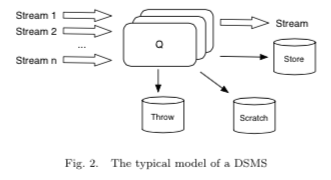
\includegraphics[width=0.75\linewidth]{images/dsms}
	\caption[General Continuous Queries Architecture]{The Continuous queries architecture proposed in~\cite{Babu:2001:CQO:603867.603884} shows that  a set of continuous queries may produce four different outputs, as a consequences of data streams processing: the \textit{Stream}, which is composed by all the element of the answer that are produced once and never changed; the \textit{Store}, which is composed by the a part of the answer that may change; the \textit{Scratch}, which represents the working memory of the system; the \textit{Throw}, a sort of garbage collector of stream tuples.} 
  	\label{fig:dsms}
\end{figure}

Figure~\ref{fig:dsms} reports the general continuous queries architecture proposed in~\cite{Babu:2001:CQO:603867.603884}. This model aims of highlighting several architectural choices and their consequences. A DSMS is modelled as a set of standing queries $Q$ and one or more input streams, the DSMS can produce four outputs~\cite{Cugola:2012:PFI:2187671.2187677}:

\begin{itemize}
\item The \textit{Stream} - it is formed by all the elements of the answer that are produced once and never changed;
\item The \textit{Store} - it is filled with parts of the answer that may be changed or removed at a certain point in the future. 
\item The \textit{Scratch} - it represents the working memory of the system. It is exploited to store data that is not part of the answer, but that may be useful to compute the answer;
\item The \textit{Throw} - it where the used unneeded tuples are collected and throw away.
\end{itemize}

Notice that the Stream and the Store together define the current answer to queries Q.


\begin{figure}[tbh]
  \centering
	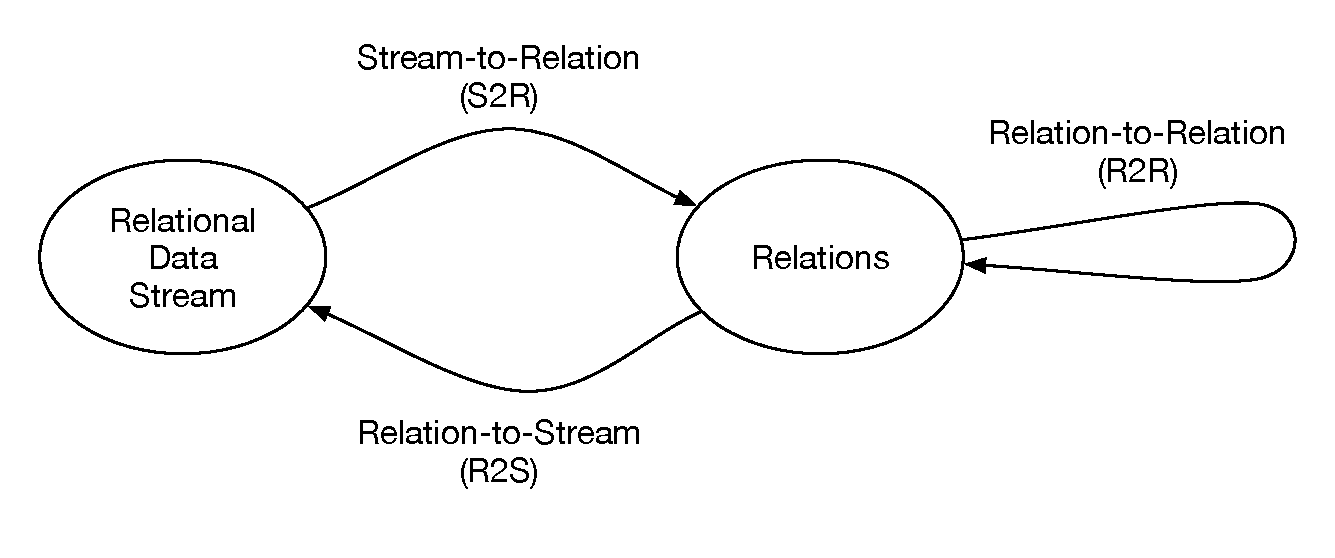
\includegraphics[width=\linewidth]{images/cql-model}
	\caption[CLQ DSMS Model]{The CLQ DSMS Model was proposed in~\cite{Arasu2006}. The S2R operator transforms the incoming Relational Data Stream, which is possibly unbounded, into a bag of timestamped data items, we call Relations. The R2R operator applies relational algebra to the existing relations in order to transform into new ones. Finally, if the relations have to be transformed back to relational data stream, the R2S operator appends the results to the output stream.} 
  	\label{fig:cql}
\end{figure}

Moreover, the DB group of the Stanford University proposed the CQL stream processing model, which defines a generic DSMS through three classes of operators~\cite{Arasu2006}.


\noindent A DSMS system is is composed by operators that are able to manage the information stream in different phases. Figure~\ref{fig:cql} gives a representation of the general model, composed by three modules that belong to three classes of operators:  

The Stream-to-Relation (S2R) is the first class of operators that manage data streams.  A stream is potentially unbounded, thus the S2R operators extracts finite bags of timestamped data items, transforming streams in relations. There are several operators of this class and the sliding window is one of the most studied. A sliding window creates a view over a portion of the stream that changes (slides) over time. Time-based sliding windows are sliding windows that create the window and slide it accordingly to time constraints: they are defined by two parameters, the width $\omega$ – i.e. the time range that has to be considered by the window – and the slide $\beta$ – i.e. how much time the window moves ahead when it slides.

The second class of operatos is the Relation-to-Relation (R2R). Relations may be transformed in another ones through relational algebraic expressions, which are applied by operators that belong to the R2R class. 

Finally, the third class of operators is the Relation-to-Stream (R2S). This kind of operators are necessary when the output of the query processor should be a stream. Every time the continuous query is evaluated, the results are processed by the R2S operator, which determines the data items it has to stream out and appends results to the output stream. There are usually three R2S operators:

\textbf{Rstream}, which streams out the computed timestamped results at each step. Rstream answers can be verbose as the same results can be computed at different evaluation times, and consequently streamed out. It is suitable when it is important to have the whole query answered at each step.

\textbf{Istream} streams out the difference between the timestamped results computed at the last step and the one computed at the previous step. Answers are usually short (they contain only the differences) and consequently this operator is used when data exchange is expensive. Istream is useful when the focus in on the results that are computed by the system.

\textbf{Dstream} does the opposite of Istream: it streams out the difference between the computed timestamped results at the previous step and at the last step. Dstream is normally considered less relevant than Rstream and Istream, but it can be useful.


\subsection{Complex Event Processing}\label{sec:cep}

The Complex Event Processing (CEP) finds its origins in the publish-subscribe domain~\cite{Eugster:2003:MFP:857076.857078}. It comes from interpreting IFP items as notifications of events which arrive from  external world. The traditional publish-subscribes systems process the incoming information flows one event at time, applying the filtering methods at topic level or at content level and evaluating the event relevance w.r.t the subscribers. 

\begin{figure}[tbh]
  \centering
	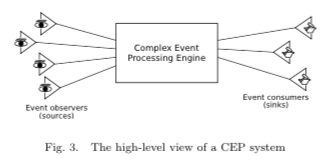
\includegraphics[width=0.75\linewidth]{images/cep}
	\caption[General CEP Model]{The CEP model in figure is proposed in~\cite{Cugola:2012:PFI:2187671.2187677}. It relies on the ability to identify patterns that match multiple incoming events, which are seen as notifications. The processing consist in filtering and correlating the incoming events on the basis of their content. The goal is notify to subscribed sinks the presence of a certain pattern or some ordering relationships between events. The CEP Engine output is an event stream too.} 
  	\label{fig:cep}
\end{figure}



Complex Event Processing systems, namely CEP Engines, extend this behaviour, filtering and combining the events to understand what is happening in terms of higher-level information. The CEP model focuses on detecting occurrences of particular event patterns, which actually represent the higher-level information flows. For this reason, CEP Engines increase the expressive power of the subscription language to consider complex event patterns that involve the occurrence of multiple, related events~\cite{Cugola:2012:PFI:2187671.2187677}.


Figure~\ref{fig:cep} shows the CEP Engine Model proposed in~\cite{Cugola:2012:PFI:2187671.2187677}. A CEP Engine is responsible for processing such events as explained above, in order understand what is happening in terms of higher-level information. Sinks aim to    be notified  about this new information level and thus they act as consumers of the CEP Engine output events. 
CEP Engines are designed to face the main limitation of most DSMSs: the ability to detect complex patterns of incoming items, involving sequencing and ordering relationships.

\section{Stream Reasoning}\label{sec:sfp}

Answering such queries like \textit{What are the top 10 emerging topics under discussion on Twitter, Facebook and Goolge+ and who is driving the discussions?} requires systems that can manage rapidly changing worlds at the semantic level. \textbf{Stream Reasoning} is a novel research trend focused on combining DSMSs, which can analyse data on the fly (see Section~\ref{sec:dsms}) and reasoners, which can perform such complex reasoning tasks (see Section~\ref{sec:sw}), in order to make possible reasoning on rapidly changing information.

%A first step toward stream reasoning~\cite{DBLP:conf/fis/ValleCBBC08} tries to combine the power of existing data stream management systems and the Semantic Web. In the context LarKC European Research Project\footnote{http://www.larkc.eu}~\cite{4597242, 4120457} was proposed a pluggable algorithmic framework for a such a system, which includes the following steps:
%\begin{itemize}
%\item[1.] \textit{retrieve} relevant resources from the incoming input stream by a selection step, where the information is filtered
%\item[2.] \textit{abstract} by extracting information, calculating statistics and transforming from fine grain data streams into aggregated events.
%\item[3.] \textit{select} relevant problems/methods/data;
%\item[4.] \textit{reason} upon the aggregated knowledge; 
%\item[5.] \textit{decide} on the base of some decision criteria, defined by the application developer, if the quality of the answer is good enough or if a new iteration is needed.
%\end{itemize} 


\subsection{RDF Stream}\label{sec:rdfstream}

Traditional DSMS system work with relational data stream, as the CQL general model in Figure~\ref{fig:cql} reports. In the Stream Reasoning context the data streams have to be semantically processed. Thus, the information flows require a semantic consolidation, which must consider both performances and expressiveness. We focus \textit{RDF streams}, which are data streams where the data items are modelled through RDF~\footnote{Cf. \url{http://www.w3.org/TR/2004/REC-rdf-primer-20040210/}.}. 

For example, let's consider the following stream: at time 1, an event $e_1$ states that an article \textit{:paper$_1$} is written by \textit{:alice}, while at time 5, a data item $e_2$ states that \textit{:paper$_2$} is written by \textit{:bob}. The stream $((e_1,1),(e_2,5))$ can be represented by the following RDF stream:
\[\textit{(:paper$_1$ ub:publicationAuthor :alice), 1}\]
\[\textit{(:paper$_2$ ub:publicationAuthor :bob), 5}\]

Initial works on RDF Stream formalisation have proposed two alternative formats for the Stream consolidation~\cite{DBLP:conf/fis/ValleCBBC08}:
\begin{itemize}
\item RDF molecules stream - it is an unbounded bag of pairs $< \rho, \tau >$, where $\rho$ is a RDF molecule~\cite{TrackingMolecules} and $\tau$ is the timestamp that denotes the logical arrival time of RDF molecule $\rho$ on the stream;
\item RDF statements stream, is a special case of RDF molecules stream in which $\rho$ is an RDF statement instead of an RDF molecule  .
\end{itemize} 

The single RDF statement representation for events was exploited in different works ~\cite{Barbieri2010,Lephuoc2011}, while more recent researches~\cite{DBLP:conf/semweb/BalduiniVDTPC13} are studying the cases where events are modelled through RDF graphs (i.e. set of RDF statements). 

The  RDF stream  definition is based on the relational data stream one. \textit{RDF streams are sequences of timestamped data items, where a data item is a self- consumable informative unit}. Some the main characteristics of relational data streams still hold~\cite{DBLP:conf/pods/BabcockBDMW02}, thus RDF Stream are:
\begin{itemize}
\item \textbf{continuous}: new data items are continuously added to the stream;
\item \textbf{potentially unbounded} : a data stream could be infinite;
\item \textbf{transient}: it is not always possible to store data streams in secondary memory;
\item \textbf{ordered}: data items are intrinsically characterised by recency.
\end{itemize}

\subsection{Continuous Extensions of SPARQL}\label{sec:continuous-sparql}

There are many extension of SPARQL, which extends the SPARQL 1.1 (see Section~\ref{sec:sparql}) to include continuous operators (see Section~\ref{sec:dsms}):

Continuous SPARQL (C-SPARQL)  is a language for continuous queries over streams of RDF data that extends SPARQL 1.1~\cite{Barbieri:2010:QRS:1860702.1860705}.

For instance, the following C-SPARQL query asks to report every day the people mentioned during the last week in the stream of those who have published a paper:

\begin{center}
\raggedright
\textit{SELECT ?person}\\
\textit{FROM STREAM $<$http://www.ex.org/lubm-stream$>$ [RANGE 1w STEP 1d]}\\
\textit{WHERE \{?person a ub:Person\}}\\
%\textit{UNDER RDF ENTAILMENT REGIME}
\label{code:query-bg}
\end{center}
Query:~\ref{code:query-bg}: Example of C-SPARQL QUERY.\\

The requested information is not explicitly stated, but being the range of the \textit{ub:publicationAuthor} property a \textit{ub:Person}, an RDFS reasoner can deduce it and, thus, it can allow to answer the query.

Another example is CQELS-QL~\cite{Lephuoc2011} – a declarative query language built from SPARQL 1.1 grammar. As C-SPARQL, it extends SPARQL with operators to query streams. The main difference between C-SPARQL and CQELS-QL is in the R2S operator supported: CQELS-QL supports only Istream, whereas C-SPARQL supports only Rstream. 

Last but not least, SPARQLstream~\cite{Calbimonte:2010:EOA:1940281.1940289} is another extension of SPARQL used in Morph$_{stream}$. Unlike CQELS and the C-SPARQL Engine, SPARQLstream supports all the streaming operators presented in Section 2.3.4. 

\subsection{RDF Stream Processing Engine}\label{sec:rspengine}

\begin{figure}[tbh]
  \centering
	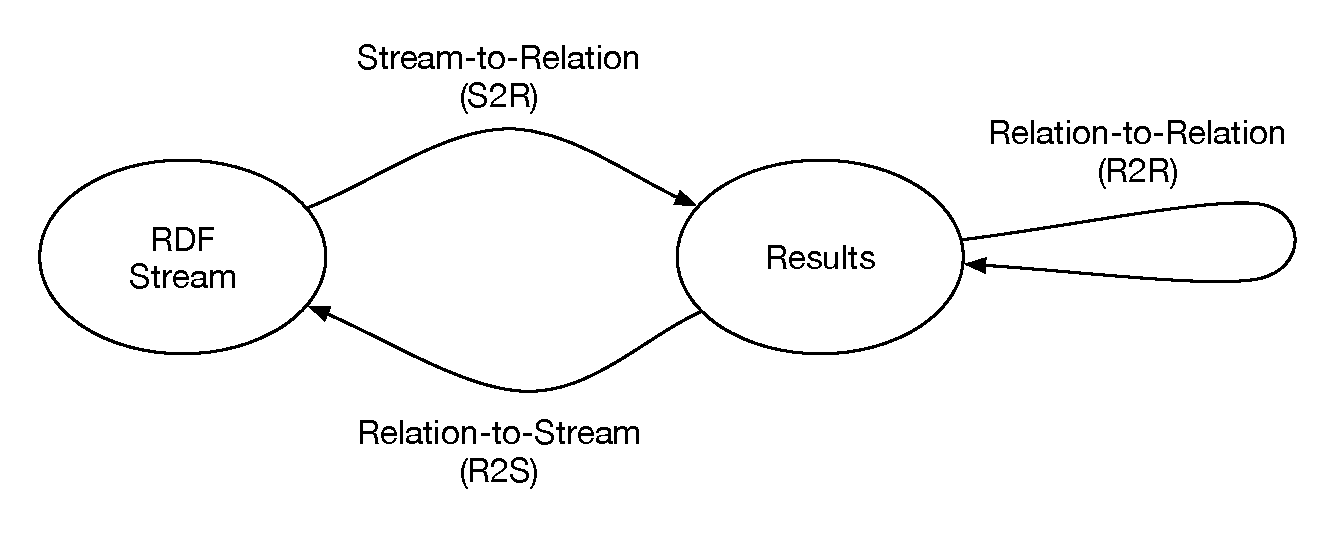
\includegraphics[width=\linewidth]{images/rsp-engine-model}
	\caption[RSP Engine Model]{This RSP Engine model is inspired to the CQL DSMS Model proposed in~\cite{Arasu2006} and reported inf Figure~\ref{fig:cql}. The incoming relation stream is now an RDF Stream. The S2R operator is usually implemented with a sliding window, which logically selects a portion of the RDF Stream. The evaluation of the continuous queries represents the R2R operator. The RSP Engine transforms the queries results back into an RDF Stream, applying the R2S operator.} 
  	\label{fig:rsp-engine-model}
\end{figure}

Sections above report that RDF Stream Processing has three basic building blocks: 1) RDF streams, we introduced in Section~\ref{sec:rdfstream} 2) continuos extensions of SPARQL, like the ones we briefly described in Section~\ref{sec:continuous-sparql}, and 3) reasoning algorithms able to cope with rapidly changing information.

Collectively, IFP Engines that process RDF streams using those SPARQL extensions and reasoning algorithm are known as \textbf{RDF Stream Processing} (RSP) \textbf{Engines}.

Among RSP Engines, we target window-based RSP Engines, i.e. processors whose \textbf{continuous query language} allows to open sliding windows to capture segments of RDF streams. The C-SPARQL Engine\footnote{\url{https://github.com/streamreasoning/CSPARQL-engine}}, Sparkwave~\cite{DBLP:conf/debs/KomazecCF12}, CQELS~\cite{Lephuoc2011}, and Morph$_{stream}$~\cite{DBLP:journals/ijswis/CalbimonteJCA12}  are examples of window-based RSP Engines. The first two processes C-SPARQL~\cite{Barbieri2010}, continuous queries, where as the second two proposes their own extensions (respectively, CQELS-QL and SPARQL$_{stream}$). The first two can also process C-SPARQL queries under RDFS entailment regime\footnote{\url{http://www.w3.org/TR/sparql11-entailment/#RDFSEntRegime}}. 
Morph$_{stream}$ uses Ontology-Based Data Access techniques for the continuous execution of SPARQLstream queries against virtual RDF streams that logically represent relational data streams.

The logical processing model of RSP Engines in Figure~\ref{fig:rsp-engine-model} follows the one initially proposed in DSMS (see Figure~\ref{fig:cql}).

The following three logical steps\footnote{Physical evaluation may differ from this logical steps.} compose such model: 
\begin{itemize}
\item[1.] A portion of the RDF stream is logically selected using a sliding window operator; This is the \textbf{stream-to-relation} step. 
\item[2.] The WHERE clause of the query is evaluated (including the possibly required reasoning tasks) and a sequences of results are produced, this is the \textbf{relation-to-relation} step.
\item[3.] Results are transformed back in timestamped elements and are appended to the output, this is the \textbf{relation-to-stream} step 
\end{itemize}

Figure~\ref{fig:rsp-engine-schema} proposes a block schema for RSP Engines, with the aim to clarify the general process presented in Figure~\ref{fig:rsp-engine-model}. The schema disposes the S2R, the R2R and the R2S operators into a pipeline, drawing the RDF Stream path through the RSP Engine.


\begin{figure}[tbh]
  \centering
	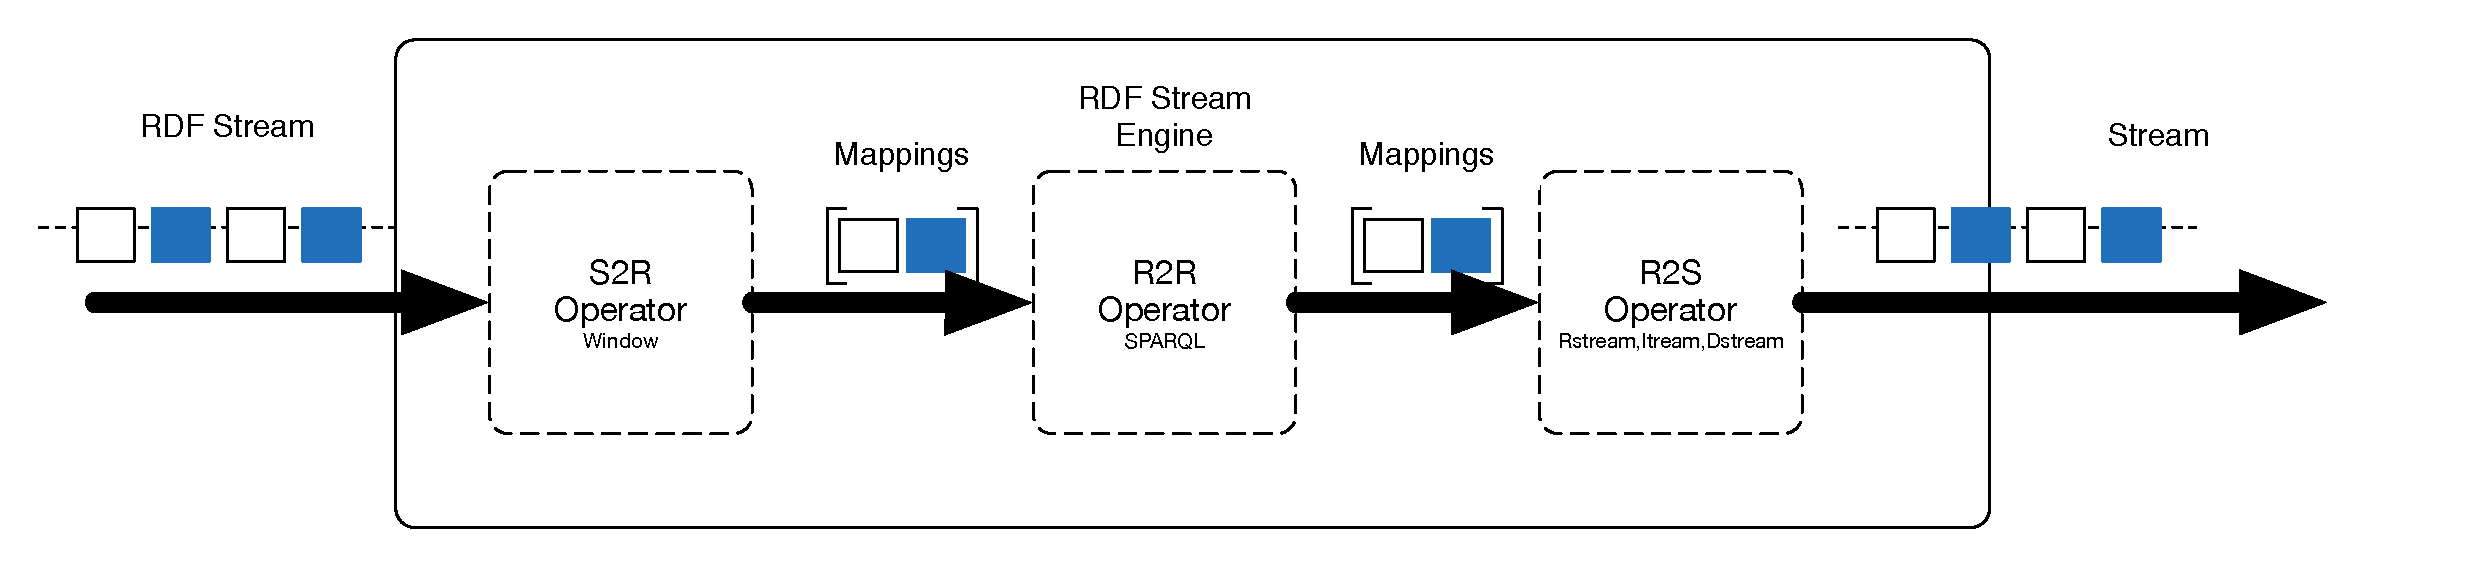
\includegraphics[width=\linewidth]{images/rsp-block-schema}
	\caption[RSP Engine Block Schema]{This block schema translates the general RSP Engine model presented in Figure~\ref{fig:rsp-engine-model}. It disposes each RSP Engine operator into a pipeline, clarifying the RDF Stream path: it is transformed into a set of relations upon which it is possible to perform continuous queries (S2R); the R2R operator applies a relation algebra which can handle data stream and produces new relations, then the query results are transformed back into an RDF Stream (R2S).}
  	\label{fig:rsp-engine-schema}
\end{figure}

\pagebreak

\section{Empirical Research}\label{sec:empirical-research}

The problem of understating the nature of the Computer Science (CS) research has one stronghold in Tichy's work of 1995~\cite{Tichy:1995:EEC:209090.209093}. He and his collaborators evaluated 400 articles published in 1993, randomly selecting papers form ACM and from a few journals in Systems and Software Engineering. Tichy's research had the aim of classify Computer Scientist research habits. He proposed the following taxonomy~\cite{Tichy:1995:EEC:209090.209093} for the classification of the CS research works:
\begin{itemize}
\item \textit{Formal theory}: theorems and their proofs, which provide formally tractable main contributions. 
\item \textit{Design and modelling}:  techniques and methods definition, models design and their implementation. Works like  software tools or performance prediction models provide a contribution that cannot be proven formally.
\item \textit{Empirical work}: collection, analysis and observations about known techniques, systems, or models, or about abstract theories or subjects. The contribution of these works focuses on evaluation.
\item \textit{Hypothesis testing}: hypotheses definition and the design of experiments for their verification. The contribution of these papers is opening new research scenarios.
\item \textit{Others}: articles that do not fit any of the four categories above.
\end{itemize}

Tichy's evaluation showed that, despite the engineering epistemology of the majority of the evaluated paper, there was a deficiency in term of empirical evaluation w.r.t model \textit{Design and Modelling} works. Researchers prefer to focus on the proposal of new models and their implementation rather than evaluating the existing ones. More recent works~\cite{Wainer:2009:EEC:1518331.1518552} observe and confirm Tichy's observations: the amount of evaluation reported in the Computer Science papers is still low.

Practically, an empirical study requires to define experiments for testing one or multiple systems. Comparing different results allows to distinguish what we believe it is truth from what we observe. The empirical evaluation has the aim of supporting the scientific method and rather plays a fundamental role in other research fields.

Software Engineering (SE) and many other Computer Science research areas have failed to produce the models and analytical tools that are common in other sciences~\cite{Perry:2000:ESS:336512.336586}. CS research lacks the knowledge about the mechanisms which drive the costs and benefits of software tools and methods, making hard to understand whether analysis are based on faulty assumptions or the new evaluation methods are properly.

It is important to remember that empirical studies can be used not only retrospectively to validate systems or idea after they have been implemented, but also proactively to direct the research. Formal experiments, case studies and prototyping exercises are all adequate empirical studies. Independently from their form, they are a key way to fill the lack and sustains with credible observations those CS research fields which requires an evaluation of the proposals. Indeed empirical studies allow to learn something useful by comparing theory to reality through the following steps~\cite{Perry:2000:ESS:336512.336586}:
\begin{itemize}
\item  formulating an hypothesis or question to test
\item  observing a situation
\item  abstracting observations into data
\item  analysing the data
\item  drawing conclusions with respect to the tested hypothesis
\end{itemize}
\pagebreak

\section{Software Testing}\label{sec:software-testing}
Software Testing (ST) techniques start with the intent of finding software bugs and ends with methods to evaluate system behaviour under testing conditions. In general ST is an investigation over software products to evaluate the software quality. According to IEEE Standards ~\cite{IEEEStd610.12-1990:glossary} there are two basic classes of software testing, black box testing and white box testing: 

\begin{itemize}
\item Black box testing [BBT] - it ignores the internal mechanisms of a system or component and focuses solely on the outputs
generated in response to selected inputs and execution conditions.
\item White box testing [WBT] - is takes into account the internal mechanism of a system or component. 
\end{itemize} 

Black-box testing  methods  examine the functionality of a system without peering into its internal structures or workings. BBT exploits test cases built around specifications and requirements of the software. An external descriptions of the software is mandatory, and it must also include software specifications, requirements and design parameters.  The test designer selects both valid and invalid inputs and determines the correct output without any knowledge of the test object's internal structure.

White-box testing  method instead exploits complete knowledge about software internal structures. In WBT an internal perspective of the system is required to design test cases. The test designer analyses the code, understands the expected output and chooses many inputs to properly exercise the paths he has found. 

The ST sub-field which tries to offer an objective and independent view of the software is Software Performance Testing (SPT), defined as  \textit{testing conducted to evaluate the compliance of a system or component with specified performance requirements}~\cite{IEEEStd610.12-1990:glossary}. SPT requires to identify the key transactions and their data requirements. Once it is done, the test designer creates a number of different types of tests, in order to evaluate software performance w.r.t test variations. The design of the test follows the researcher needs about metrics evaluation. The choice depends on the nature of the application and how much time is available for performance testing. The following testing terms are generally well known in the industry~\cite{Molyneaux:2009:AAP:1550832}:

\begin{itemize}
\item \textit{Load testing} - it is the simplest form of performance testing, its aim is to understand the behaviour of the system under an expected load (the load kind depends on the software system). Moreover, it points to meet performance targets for availability, concurrency or throughput, and response time. This test will give out the response times of all the critical transactions and it can point out bottlenecks in the application software. Load testing is the closest approximation of real application use.

\item \textit{Stress testing} -  it is used to understand the upper limits of capacity of a system and determine the system's robustness in terms of extreme load. A stress test may causes the application or some part of the supporting infrastructure to fail. The results of this kind of test are  capacity measure as much as performance. It's important to understand software limitations, in order to face future growth of application traffic, which may be hard to predict.

\item \textit{Soak testing} - it is performed to determine if the system can sustain the continuous expected load. It essentially involves applying a significant load to a system for an significant period of time. The goal is to discover how the system behaves under sustained use or identify steady state conditions. During soak tests, memory utilization is monitored to detect potential leaks. Also important, but often overlooked is performance degradation, i.e. to ensure that the throughput and/or response times after some long period of sustained activity are as good as or better than at the beginning of the test. 
\end{itemize} 
\pagebreak
\section{Benchmarking}\label{sec:benchmarking}

Benchmarking is the primary method for measuring the performance of a systems, hardware or an application. Indeed a benchmark is a procedure, problem, or test that can be used to compare systems or components to each other or to a standard~\cite{IEEEStd610.12-1990:glossary}. Thus, benchmark results are used to evaluate the performance of a given system on a well-defined workload~\cite{Menasce:2001:CPW:560806}.

Many benchmark tests exist to evaluate a wide variety system or applications under different types of workloads. The user groups like the Transaction Processing Performance Council (TPC) \footnote{http://www.tpc.org/information}, a non-profit corporation founded to define transaction processing and database benchmarks, or analogues corporations are useful resources of be informed about updated types of benchmarks. 

Generic benchmarks allows the quantitative comparison of system performances or price/cost. In database context performance is typically a throughput metric (work/second) and price is typically a five-year cost-of-ownership metric~\cite{DBLP:books/mk/Gray93}. The quantitative comparison requires the benchmark to be run on several different systems and to record each system is measurements.  The estimation evaluated from results is usually the relative system performance, because the cost of implementing and measuring a specific application on many different systems is almost always prohibitive.

\subsection{Domain Specifc Benchmarks}  \label{sec:tcp}

A single metric can not measure the performance relative to all applications of a computer systems~\cite{DBLP:books/mk/Gray93}. Performances depend strictly on the application domain, because each system is designed for a few problem in a domain and may be inadequate to perform other tasks.

It is worth to note the work of Jim Gray about Domain-specific benchmarks~\cite{DBLP:books/mk/Gray93}, a kind of benchmarking methods and tools  which responds to computer system diversity. A Domain-specific benchmark specifies a synthetic workload characterising typical applications in that problem domain. 

In order to distinguish among several solutions and workload, Gray states four key criteria that a Domain-Specific Benchmark must meet to be useful. It must be:
\begin{itemize}
\item Relevant: It must measure the peak performance and price/performance of systems when performing typical operations within that problem domain.
\item Portable: It should be easy to implement the benchmark on many different systems and architectures.
\item Scalable: The benchmark should apply to small and large computer systems. It should be possible to scale the benchmark up to larger systems, and to parallel computer systems as computer performance and architecture evolve.
\item Simple: The benchmark must be understandable, otherwise it will lack credibility.
\end{itemize} 

\subsection{Reasoning Benchmarks}\label{sec:lubm}

The number of different reasoners available is increasing and many of them are already commercial solutions. Usually, reasoners are able to process very expressive ontology languages, which can represent rather complete knowledge. However, there is an high demand of less expressive ontology languages, which are less expensive in term of reasoning or other computational tasks. Commercial reasoners try to solve the issue called \textit{computational cliff}. They face the trade-off between \textit{complexity and expressiveness} versus \textit{scalability}. Benchmarking tools are useful to evaluate reasoning system w.r.t. ontology languages~\cite{bock2008benchmarking}, and the most important one is the Lehigh University Benchmark (LUBM)~\cite{Guo2005}. This work proposes a  method for benchmarking Semantic Web knowledge base systems and provides an example of such a benchmarks.

Reasoning benchmarking environment requires:
\begin{itemize}
\item Ontology: LUBM exploits a synthetic ontology named Univ-Bench\footnote{http://www.lehigh.edu/~zhp2/2004/0401/univ-bench.owl}, which describes universities, departments and the activities that occur at them. The popularity of OWL is high many benchmarking tools allow testing performance with new ontologies~\cite{gardiner2006automated}.

\item Workload: LUBM provides a random data generator, called UBA (Univ-Bench Artificial data generator), which creates extensional data over the Univ-Bench ontology~\cite{Guo2005}.

\item Queries: LUBM comes with fourteen testing queries to stress the reasoning capabilities over the workload. LUBM contains criteria for query definition which consider for example \textit{Input size} or \textit{Complexity} to stress the reasoner and evaluate performances.
\end{itemize}

Finally. LUBM contains three metrics for reasoners evaluation, which are commonly used in also database benchmarks:
\begin{itemize}
\item \textit{Load Time} - the stand alone elapsed time for storing the specified dataset to the system;
\item \textit{Repository Size} -  the resulting size of the repository after loading the specified benchmark data into the system;
\item \textit{Query Response Time} - it similar to databases benchmarking: for each test query the evaluation consist into
  	1) Opening the repository; 2) Executing the query for 10 times and computing the average response time. 3) Closing the repository
\end{itemize}

LUBM contains two specific reasoning metrics: \textit{Query Completeness and Soundness}: partial answering is possible in semantic web, indeed LUBM evaluate the \textit{degree of completeness of each query answer as the percentage of the entailed answers that are returned by the system}. Moreover, LUBM also provides a metric for measuring the combination of  query response time and answer completeness and soundness, to  appreciate the potential trade-off.

\subsection{DSMS \& CEP Benchmarks}\label{sec:linear-road}

The Linear Road~\cite{arasu2004linear} is a stronghold about DSMS and CEP benchmarking. It posed several challenges about IFP system benchmark design which are:
\begin{itemize}
\item  \textit{Semantically Valid Input} -  Input data can not be randomised but should have some semantic validity.
\item  \textit{Continuous Query Performance Metrics} - Standard DBMS time to completion metrics is inadequate, it must also be considered \textit{Query Response Time} and \textit{Supported Query Load}. 
\item  \textit{Results Correctness} - benchmark implementations must be validated w.r.t the registered queries to ensure that results are consistent with the benchmark specifications.
\item  \textit{Query Language Independence}: no standard query language for streaming systems exists, thus the query requirements must be language independent.
\end{itemize}
%
% Moreover, the variety of CEP and DSMS domains and the lack of standards in query languages and data formats extends these benchmark design challenges. First of all DSMS Benchmarking must consider the challenges presented in the Linear Road work:
\cite{arasu2004linear} defines the requirements a benchmarking system for IFP must fulfil according with these challenges. It provides also an implementation of a benchmark that meets all the requirements by design. The benchmark consists into a simulation of an urban highways system where toll charges are dynamically determined. The input data contains: a stream of position reports, which specify the location of a vehicle every 30 seconds; an historical query requests, which may be issued by a vehicle with some fixed probability every time it emits a position report.

Further works, like the BiCEP project\footnote{http://bicep.dei.uc.pt}, try to identify some o requirements for CEP benchmarking and they develop a synthetic benchmarking set to measure the event processing activity such systems. CEP Benchmarking are evaluated with Jim Gray criteria, we already presented in Section~\ref{sec:tcp}. 

\begin{figure}[tbh]
  \centering
	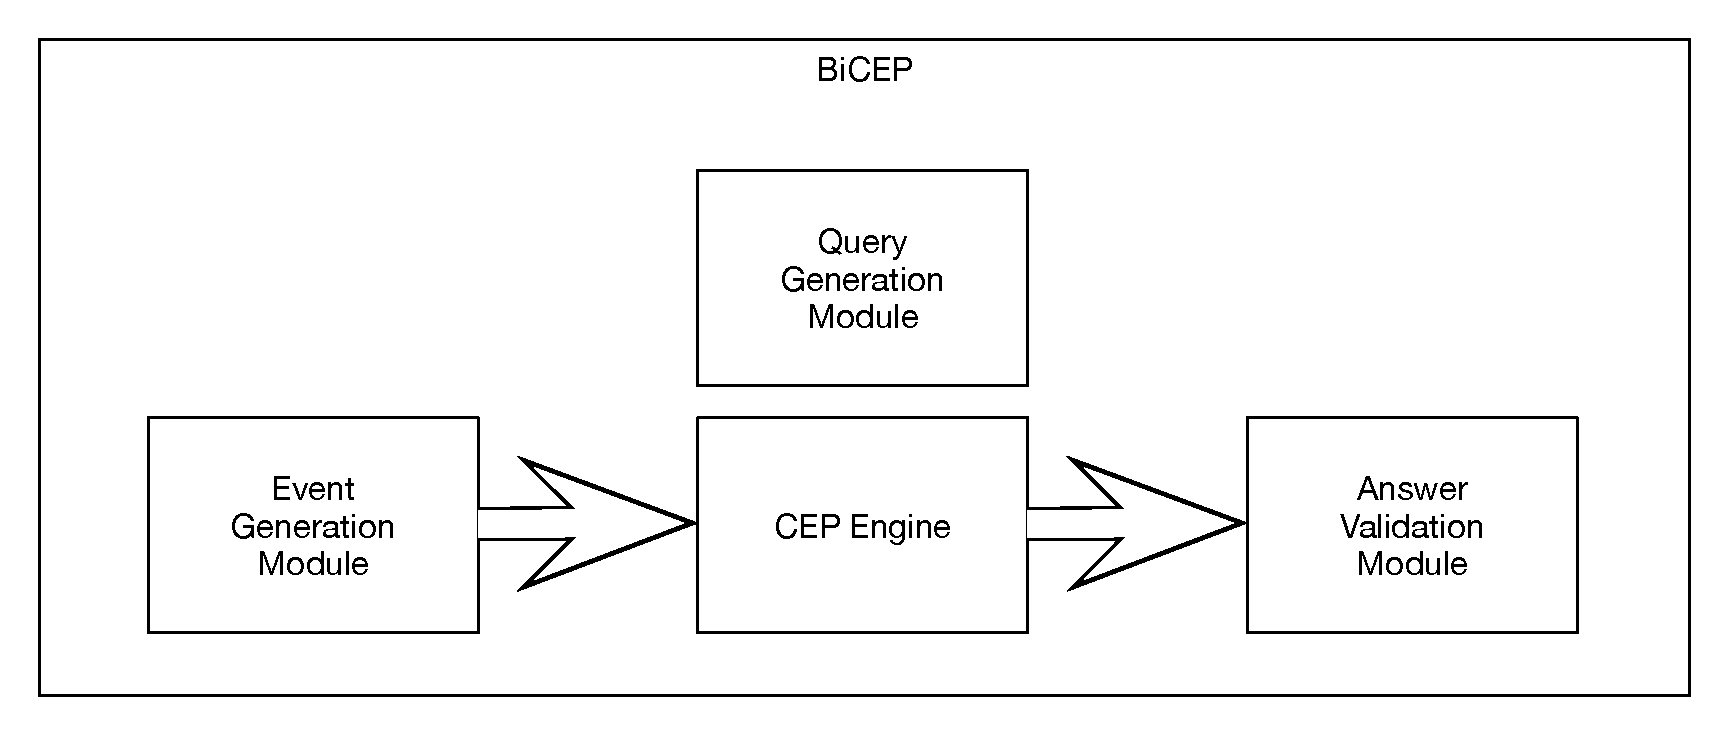
\includegraphics[width=\linewidth]{images/bicep_schema}
	\caption[BiCEP Benchmarking Schema]{BiCEP Benchmarking Schema proposed in~\cite{bizarro:DSP:2007:1143}. \textit{The Event Generator Module} produces the input consumed by the \textit{CEP Engine} through the application of the queries provided by the \textit{Query Generation Module}. The \textit{Answer Validation Module} consumes \textit{CEP Engine} results and states their validity. The CEP Engine interface ensures that any pre processing of the incoming events is part of the performance measurement.} 
  	\label{fig:bicep-schema}
\end{figure}

BiCEP project presents an first schema model for a CEP Engine benchmarking system. Figure~\ref{fig:bicep-schema} displays the schema: the input data are generated by the Event Generator Module; the CEP Engine results are consumed by the Answer Validation Module. Figure~\ref{fig:bicep-schema} shows also the CEP Engine interfaces, which ensures that any buffering, event cleaning or event transformation phase, that happens at the CEP Engine, is part of the overall performance measure. 

Synthetic benchmarks offers many benefits like data availability, experimental control, and scalability. However, it is hard to develop a synthetic benchmark that is representative of such a wide range of CEP applications at the same time. BiCEP development is oriented towards a set of small domain specific benchmarks with different data sets and different queries~\cite{bizarro:DSP:2007:1143}.

Finally, BiCEP project presents a set of metrics for CEP benchmarking, the most relevant ones in performance evaluation context are: \textit{Response time}: the time since the last event of some event pattern is fed into the system until the system notifies the event pattern detection. \textit{Scalability} in order to compare system with different scale levels; \textit{Adaptivity}. the system response to input variation, which is mandatory because CEP system rarely face stable input streams.

\subsection{RDF Stream Processing (RSP) Benchmarks}\label{sec:sr-benchmarking}

RSP Engines are a clearly example of complex systems that face heterogeneous domains of application. This should be enough to follow the Tichy's suggestion and start their empirical evaluation. Moreover, the number of implemented RSP Engines is increasing, but the works about their evaluation are still limited and do not address properly the definition of the key performance indicators (see Section~\ref{sec:sfp}), making harder any comparison of the different systems.

Recent works on RSP benchmarking try to follow the Linear Road example, posing the main challenges for the SR benchmarking and developing them one by one into Seven Commandments for RSP Engine benchmarking~\cite{DBLP:conf/esws/ScharrenbachUMVB13}.

In the following we report the these commandments as they are described in~\cite{DBLP:conf/esws/ScharrenbachUMVB13}:
 
RDF Stream Processing Engines must implement good strategies for \textit{Load Balancing} [S.1], because they usually consider several input information streams with possible bursts. It is possible to stress the system under various conditions by repeatedly applying a set of changes to the input.

A stress test is required to measure the performance of \textit{Flow Data Joins And Inference} [S.2]. It has to consider increasingly complex cascades of joins in order to design the stress test for Simple joins, which put no further constraints on the join but on the join-equality. The benchmark has to add further constraints on the joins, and subsequently to the data. In this way is possible: (i) enabling the testing og Sequential joins, which add a sequential constrains;  (ii) allowing the testing of Temporal joins, which extend sequential joins by enabling advanced temporal constraints. On the other and, \textit{joining stream and background data} [S.3] always results in simple joins. A stress-test must consider single joins and increasingly complex cascades.

The benchmark must test \textit{Aggregates} [S.4], which enable counts, averages and any other arithmetic operation on groups of entities or literals. Moreover, it must take count of properly groups scaling: group number, group complexity or tuning the data to provide a big number of candidate, but a small number of selected groups.

In distributed settings, an RSP benchmark must ensure the correctness of query answers, handling \textit{Unexpected Data} [S.5] like out-of-order arrival of information and data loss. A benchmark should be able to measure this ability evaluating precision and recall of the amount of missing data with two tests, (i) by increasing the number of out-of-order events or (ii) by testing how long and how many data can be handled until some nosily data observation will be no longer considered for processing.

A benchmark has two possibility for stressing the system through \textit{Schema} [S.6] variations: (a) Evaluating the system ability to handle an increasing number of axioms in system ontology. (b) Changing statements that generate a more complex reasoning. It is important to know that: the axioms extension proposed by (a) could not have been deduced from existing ones and that the changes proposed by (b) may stress an RSP system significantly if they increase the expressive power of the schema, not only for the background data but also of the data flow.

Finally, a benchmark should evaluate an RSP Engine through \textit{Changes in Background-Data} [S.7]. Any stress test on background data changes should variate the update frequency and the entire amount of data involved in the update, forcing the system to access background-data from disk as much as possible.

Implemented proposals for RSP benchmarking has been published, but none of them impacts the community as the Linear Road did for DSMSs. More careful analysis of those solutions, presented in the following section, evidence some lacks w.r.t the commandments proposed in~\cite{DBLP:conf/esws/ScharrenbachUMVB13} 

\subsubsection{SRBench}\label{sec:srbench}

SRBench is presented as \textit{a general-purpose benchmark primarily designed for streaming RDF/SPARQL Engines and based on real-world data sets}~\cite{Zhang2012}. The SRBench dataset is composed by: the LinkedSensorData, which  is a real-world data set containing the US weather data published by Kno.e.sis\footnote{ http://knoesis.wright.edu};  GeoNames and DBpedia data sets, which allow to demonstrate the ability of the benchmarked system to deal with interlinked data.

Moreover,~\cite{Zhang2012} provides some relevant metrics to evaluate the performance of the system: 
\begin{itemize}
\item \textit{Correctness of the query results} - it must be validated and the validation results should be expressed in terms of precision and recall.
\item \textit{Throughput} - it is defined as limit number of incoming data an RSP system is able to process per time unit.
\item \textit{Scalability} - it means evaluating how the system reacts to an increasing number of incoming streams and variation on number of registered continuous queries.
\item \textit{Response time} - it is the amount of time between a data item enters the system and the RSP Engine outputs the query results.
\end{itemize}

SRBench provides a query set composed by seventeen queries, which are designed upon a real use case in LSD. The queries vary involving single or multiple input streams, in order test many properties of RSP Engines. They cover the most important SPARQL operators and the common streaming SPARQL extensions and several queries require RDFS reasoning.

SRBench was criticised w.r.t. proposed commandments above~\cite{DBLP:conf/esws/ScharrenbachUMVB13}. It only cover [S.3] and [S.6] but with some limitations: the queries are fixed and thus do not allow an exhaustive assessment of join performance required by [S.3]. Testing variations of the expressive power is possible in SRBench, but it was not done yet as demanded by [S.6]. The commandments [S.2] and [S.4] are partially satisfied. The SRBench provides data and use-cases for sequential joins but it does not implement stress tests for temporal joins [S.2]. About [S.4], SRBench tests the aggregates only through single queries. The other commandments are not cover yet, even if some of them were marked as potential extensions of the current SRBench implementation. In~\cite{DBLP:conf/esws/ScharrenbachUMVB13}, Table 1 summarises which features SRBench fulfil, which not, and which are only potential.

\subsubsection{LSBench}\label{sec:lsbench}

LS Bench proposes methods that enables meaningful comparisons of RSP processing Engines and a framework that provides several customisable tools for simulating realistic data, running engines, and analysing the output. LSBench also includes three tests to evaluate the RSP stream Engines~\cite{DBLP:conf/semweb/DellAglioCBCV13}:
\begin{itemize}
\item A functional test to verify the operators and the functionalities supported
by the engines, similar to SR Bench.
\item A correctness test is to verify if the tested RSP Engine produces the correct output. Actually the test assumes that the content of the output is correct, and it analyses only the number of produced answers.
\item A maximum input throughput test, whose aim is evaluating the maximum throughput of the RSP Engine, by increasing the data streak rate and checking the number of the answers
\end{itemize}

\cite{LePhuoc2012c} provides a data generator system for benchmarking, the S2Gen, which creates data set according to the \textit{Social Network Data Stream Logic Schema}, presented again in Figure 1 of~\cite{LePhuoc2012c}. S2Gen allows to tune three parameters which influence the data generation task: 1) \textit{Generating period}, the period in which the social activities are generated; 2) Maximum number of posts/comments/photos for each user per week 3) the \textit{Correlation probabilities}: there are various parameters for the data correlations which can be customized to specify how data is related according to each data attribute.

Finally, LSBench~\cite{LePhuoc2012c} provides for each test a set of 12 fixed queries. The queries in the set vary to address different features of the engines. 

The Seven commandments for RSP benchmarking are not completely covered by LS Bench (see~\cite{DBLP:conf/esws/ScharrenbachUMVB13} Table 1). LSBench cover [S.3], but fixed queries do not allow to stress the system properly with the aim of evaluate join performances. [S.2] is only partially supported, because, LS Bench does not support stress testing for temporal joins but only for sequential. [S.4] is again only partially fulfilled: LS Bench tests aggregates only implementing single queries~\cite{DBLP:conf/esws/ScharrenbachUMVB13}.

\subsubsection{Benchmarking Query Result Correctness: CSRBench}

Further works on correctness of the RSP Engine operational semantics, showed how this variates on different implementations and influence the query results correctness~\cite{DBLP:conf/semweb/DellAglioCBCV13}.

All Stream Reasoning benchmarks presented above have a common limitation: they do not check the correctness of output produced by the benchmarked RDF Engine. SRBench verifies only through functional tests the query language supported by the engines while, LSBench does not check the answers correctness, but it limits the analysis to the number of outputs. 
SR Bench and LS Bench make two assumptions on the tested systems which may be considered erroneous: (i) they work correctly; (ii) They all have the same operational semantics. However, these assumptions do not hold for RSP Engines in general and hence these benchmarks may supply misleading information about them.
 
An extension of the SR Bench for correctness checking, CSRBench, was proposed in~\cite{DBLP:conf/semweb/DellAglioCBCV13}. It takes into account the issues that affect query results in their three main dimensions: system, query and input stream data. It includes in the benchmark three new types of parametrised queries, with the aim of stressing the S2R operators. Finally, it provides an oracle that generates and compares results of RDF stream processors and check their correctness.